\documentclass[14pt, a4paper]{extarticle}
\usepackage{GOST}
\usepackage{array}
\usepackage{verbatim}
\usepackage[detect-all]{siunitx}
\usepackage{amsmath}
\usepackage{amssymb}
\usepackage[utf8]{inputenc}
\usepackage{hyperref}
\usepackage{tempora}

\makeatletter
\renewcommand\@biblabel[1]{#1.}
\makeatother

\usepackage{listings}
\lstset{ 
	language=[Sharp]C,                 % выбор языка для подсветки (здесь это С)
	%basicstyle=\small\sffamily, % размер и начертание шрифта для подсветки кода
	keywordstyle=\color{blue}\textbf,
	numberstyle=\scriptsize\color{gray},
	numbers=left,               % где поставить нумерацию строк (слева\справа)
	numberstyle=\tiny,           % размер шрифта для номеров строк
	stepnumber=1,                   % размер шага между двумя номерами строк
	numbersep=5pt,                % как далеко отстоят номера строк от подсвечиваемого кода
	showspaces=false,            % показывать или нет пробелы специальными отступами
	showstringspaces=false,      % показывать или нет пробелы в строках
	showtabs=false,             % показывать или нет табуляцию в строках
	frame=single,              % рисовать рамку вокруг кода
	tabsize=2,                 % размер табуляции по умолчанию равен 2 пробелам
	captionpos=t,              % позиция заголовка вверху [t] или внизу [b] 
	breaklines=true,           % автоматически переносить строки (да\нет)
	breakatwhitespace=false, % переносить строки только если есть пробел
}


\usepackage{pgfplots}
\usepackage{filecontents}
\usetikzlibrary{datavisualization}
\usetikzlibrary{datavisualization.formats.functions}

\begin{document}
	
\begin{table}[ht]
	\centering
	\begin{tabular}{|c|p{400pt}|} 
		\hline
		\begin{tabular}[c]{@{}c@{}} 
\includegraphics[scale=1]{source/b_logo.jpg} \\\end{tabular} &
		\footnotesize\begin{tabular}[c]{@{}c@{}}\textbf{Министерство~науки~и~высшего~образования~Российской~Федерации}\\\textbf{Федеральное~государственное~бюджетное~образовательное~учреждение}\\\textbf{~высшего~образования}\\\textbf{«Московский~государственный~технический~университет}\\\textbf{имени~Н.Э.~Баумана}\\\textbf{(национальный~исследовательский~университет)»}\\\textbf{(МГТУ~им.~Н.Э.~Баумана)}\\\end{tabular}  \\
		\hline
	\end{tabular}
\end{table}
\noindent\rule{\textwidth}{4pt}
\noindent\rule[14pt]{\textwidth}{1pt}
\hfill 
\noindent
\makebox{ФАКУЛЬТЕТ~}%
\makebox[\textwidth][l]{\underline{~«Информатика и системы управления»~~~~~~~~~~~~~~~~~~~~~~~~~~~~~~~~~}}%
\\
\noindent
\makebox{КАФЕДРА~}%
\makebox[\textwidth][l]{\underline{~«Программное обеспечение ЭВМ и информационные технологии»~}}%
\\

\begin{center}
	\vspace{1.5cm}
	{\bf\huge Расчетно-пояснительная записка\par}
	{\bf\Large к курсовому проекту\par}
	\vspace{0.7cm}
\end{center}
 
\noindent
\makebox{\large{\bf Тема:}~~~}
\makebox[\textwidth][l]{\large\underline{~Моделирование изображений облаков~}}\\

\noindent
\makebox{\large{\bf Дисциплина:}~~~}
\makebox[\textwidth][l]{\large\underline{~Компьютерная графика}}\\

\vspace{1.5cm}
\noindent
\begin{tabular}{l c c c c c}
	Студент      & ~ИУ7-55Б~               & \hspace{2.5cm} & \hspace{2cm}                 & &  Д.О. Склифасовский \\\cline{2-2}\cline{4-4} \cline{6-6} 
	\hspace{3cm} & {\footnotesize(Группа)} &                & {\footnotesize(Подпись, дата)} & & {\footnotesize(И.О. Фамилия)}
\end{tabular}

\noindent
\begin{tabular}{l c c c c}
	Руководитель проекта & \hspace{3.5cm}   & \hspace{2cm}                 & & ~~~~~~А.А. Павельев~~~~~\\\cline{3-3} \cline{5-5} 
	\hspace{3cm}  &                & {\footnotesize(Подпись, дата)} & & {\footnotesize(И.О. Фамилия)}
\end{tabular}

\vspace{0.6cm}
\begin{center}	
	\vfill
	\large \textit {Москва, 2020}
\end{center}

\thispagestyle {empty}
\pagebreak

% СОДЕРЖАНИЕ 
\clearpage
\tableofcontents

% ВВЕДЕНИЕ
\clearpage
\section*{Введение}
\addcontentsline{toc}{section}{Введение}
Область применения компьютерной графики не ограничивается одними художественными эффектами. Во всех отраслях науки, техники, медицины, в коммерческой и управленческой деятельности используются построенные с помощью компьютера схемы, графики, диаграммы, предназначенные для наглядного отображения разнообразной информации.\par
В наше время визуализация таких природных явлений, как ландшафт, водная поверхность, растительность, небо и облака стала важнейшей задачей. Все эти детали используются в разных сферах, например: разработка компьютерных игр, моделирование спецэффектов, создание анимации.\par
Существуют несколько алгоритмов компьютерной графики, которые решают данную задача, но чаще всего, они являются слишком ресурсозатратными. Для того, чтобы изображение выглядело более реалистичным, нужно потратить больше времени и памяти на его построение. Это является проблемой, для того чтобы создать динамическую сцену.\par
Цель данной работы - создание программного продукта, позволяющего генерировать изображения облаков.\par
Для достижения представленной цели, требуется решить следующие задачи:
\begin{enumerate}
	\item[1)] проанализировать методы генерации облаков;
	\item[2)] выбрать и/или модифицировать существующие алгоритмы трехмерной графики для визуализации трехмерного изображения;
	\item[3)] реализовать выбранные алгоритмы для создания трехмерного изображения;
	\item[4)] разработать программное обеспечение для отображения трехмерного изображения облаков.
\end{enumerate}

% АНАЛИТИЧЕСКИЙ РАЗДЕЛ
\section{Аналитический раздел}
В данном разделе представлены и проанализированы способы представления данных об облаке и ландшафте, алгоритмы генерации карты высот, удаления невидимых линий и поверхностей и алгоритмы закрасок. Также поставлена задача.

\subsection{Представление данных об облаке и ландшафте}
Существуют несколько основных принципов представления данных для хранения информации об облаках и ландшафтах:
\begin{enumerate}
	\item[1)] использование регулярной сетки высот (Карта высот - HeightMap);
	\item[2)] использование иррегулярной сетки вершин и связей, их соединяющих (т.е. хранение простой триангулизированной карты);
	\item[3)] посегментная карта высот.
\end{enumerate}
\subsubsection{Карта высот}
Данные представлены в виде двухмерного массива. Уже заданы две координаты (x, y — по высоте и ширине массива), и третья координата задается значением в конкретной ячейке, это высота. 
\begin{figure}[h!]
	\centering
	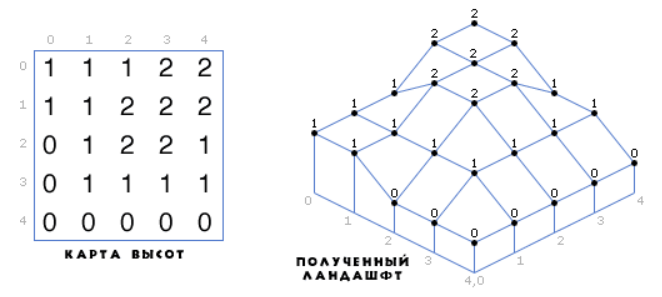
\includegraphics[scale=0.9]{source/HeightMap}
	\caption{Пример карты высот}
	\label{HeightMap}
\end{figure}
\textit{Преимущества данного принципа:} простота изменения этих самых данных, так как существует множество программ для работы с растровой графикой.\par
\textit{Минусы данного принципа:} слишком много описаний для точек, а также, в некоторых случаях, наблюдается избыточность данных.
\subsubsection{Иррегулярная сетка}
Зачастую такие решения применяются в специализированных пакетах для игр или специальных пакетах для работы с трехмерной графикой. И хранятся в виде трехмерных моделей.
\textit{Преимущества данного принципа:} используется значительно меньше информации для построения ландшафта.\par
\textit{Минусы данного принципа:} 
\begin{enumerate}
	\item[1)] сложности при динамическом освещении — вершины расположены достаточно далеко друг от друга и неравномерно; 
	\item[2)] хранение, просмотр, модификация такого ландшафта также представляет сложности.
\end{enumerate}
\subsubsection{Посегментная карта высот}
В данном способе также используются карты высот. Только вместо высот в ней хранятся индексы ландшафтных сегментов. Как эти сегменты представлены, в принципе, роли не играет. Они могут быть и регулярными, и иррегулярными.\par
\textit{Преимущества данного принципа:} возможность представления огромнейших открытых пространств.\par
\textit{Минусы данного принципа:} проблема стыковки разных сегментов и неочевидность данных.
\subsubsection{Вывод}
Наиболее эффективным принципом является использование карты высот, так как с помощью этого способа можно представлять обширные пространства, а также можно достаточно просто изменять данные.

\subsection{Генерация карты высот}
Трехмерное моделирование облаков является более реалистичным и физически точным, а также позволяет визуализировать гораздо большее число явлений, происходящих в облаках. Простым решением является использование шумовых функций для генерации карты высот. «Шумовая» функция – это псевдослучайная функция, зависящая от всех своих параметров. Для генерации карты высот чаще всего используют градиентные шумы, а именно:
\begin{enumerate}
	\item[1)] Perlin Noise;
	\item[2)] Simplex Noise.
\end{enumerate}
\subsubsection{Perlin Noise}
Шум Перлина — это градиентный шум, состоящий из набора псевдослучайных единичных векторов (направлений градиента), расположенных в определенных точках пространства и интерполированных функцией сглаживания между этими точками. Для генерации шума Перлина в одномерном пространстве необходимо для каждой точки этого пространства вычислить значение шумовой функции, используя направление градиента (или наклон) в указанной точке.\par
Алгоритм шума Перлина можно масштабировать одно-, двух- и трёхмерного вида. Более того, в алгоритм можно ввести четвёртое временное измерение, позволяя алгоритму динамически изменять текстуры во времени.
\begin{figure}[h!]
	\centering
	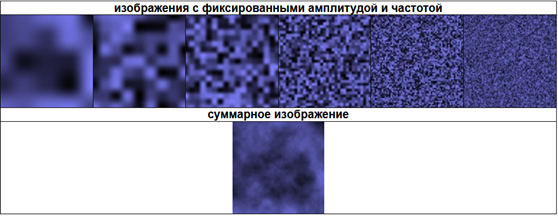
\includegraphics[scale=0.9]{source/PerlinNoise}
	\caption{Результат создания изображения с помощью шума Перлина}
	\label{PerlinNoise}
\end{figure}
\newpage
\subsubsection{Simplex Noise}
Идея данного алгоритма заключается  в том, что нужно использовать сетку из симплексов: в двумерном случае – треугольник, в трехмерном случае – тетраэдр.\par
Симплексный шум полезен для приложений компьютерной графики, где шум обычно вычисляется по 2, 3, 4 или, возможно, 5 измерениям. Для более высоких измерений n-сферы вокруг n-симплексных углов не упакованы достаточно плотно, что снижает поддержку функции и делает ее нулевой в больших частях пространства.
\begin{figure}[h!]
	\centering
	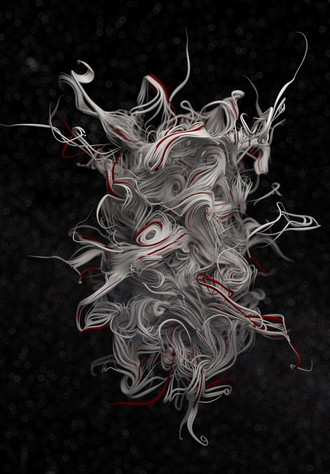
\includegraphics[scale=0.65]{source/simplex}
	\caption{Абстрактная композиция в 3D, созданная с помощью алгоритма генерации шума}
	\label{InterpolGuro}
\end{figure}
\newpage
\subsubsection{Вывод}
В качестве алгоритма для генерации карты высот был выбран шум Перлина, так как облачная поверхность обладает неравномерной структурой, но также не хаотической. Данный алгоритм достаточно прост в реализации.

\subsection{Алгоритмы удаления невидимых линий и поверхностей}
Существует несколько алгоритмов для решения данной проблемы. Необходимо провести анализ и выбрать самый подходящий для решения поставленной задачи.\par
\subsubsection{Алгоритм Робертса}
Алгоритм Робертса представляет собой первое известное решение задачи об удалении невидимых линий. Это математически элегантный метод, работающий в объектном пространстве. Алгоритм прежде всего удаляет из каждого тела те ребра, или грани, которые экранируются самим телом. Затем каждое из видимых ребер каждого тела сравнивается с каждым из оставшихся тел, для определения того, какая его часть или части, если таковые есть, экранируются этими телами.\par
\textit{Минусы данного алгоритма:} вычислительная трудоемкость алгоритма Робертса растет теоретически как квадрат числа объектов. Это в сочетании с ростом интереса к растровым дисплеям, работающим в пространстве изображения, привело к снижению интереса к алгоритму Робертса.\par
\textit{Преимущества данного алгоритма:} математические методы, используемые в этом алгоритме, просты, мощны и точны.
\subsubsection{Алгоритм Варнока} 
Алгоритм Варнока решает задачу удаление невидимых ребер и поверхностей в пространстве изображений. Идеей данного является разбиение окна на подокна, пока для каждого окна не сможем сказать, что в нем изобразить. Большая часть времени и труда затрачивается на области с высоким информационным содержимым.
\subsubsection{Алгоритм трассировки лучей}
В этом методе для каждого пикселя картинной плоскости определяется ближайшая к нему грань, для чего через этот пиксель выпускается луч, находятся все его пересечения с гранями и среди них выбирается ближайшая.\par
\textit{Преимущества данного алгоритма:}
\begin{enumerate}
	\item[1)] возможность рендеринга гладких объектов без аппроксимации их полигональными поверхностями (например, треугольниками);
	\item[2)] вычислительная сложность метода слабо зависит от сложности сцены;
	\item[3)] высокая алгоритмическая распараллеливаемость вычислений — можно параллельно и независимо трассировать два и более лучей, разделять участки (зоны экрана) для трассирования на разных узлах кластера и т. д.;
	\item[4)] отсечение невидимых поверхностей, перспектива и корректное изменения поля зрения являются логическим следствием алгоритма.
\end{enumerate}
\textit{Минусы данного алгоритма:} Серьёзным недостатком метода обратного трассирования является производительность. Метод трассирования лучей каждый раз начинает процесс определения цвета пикселя заново, рассматривая каждый луч наблюдения в отдельности. 
\subsubsection{Алгоритм, использующий Z-буфер}
Это один из простейших алгоритмов удаления невидимых поверхностей. Работает этот алгоритм в пространстве изображений. Идея z-буфера является простым обобщением о буфере кадра. Буфер кадра используется для запоминания атрибутов (интенсивности) каждого пиксела в пространстве изображения. Z-буфер – это отдельный буфер глубины, используемый для запоминания координаты z или глубины каждого видимого пиксела в пространстве изображения. По сути, алгоритм является поиском по x и y наибольшего значения функции z (x, y).\par
\textit{Преимущества данного алгоритма:} главное преимущество алгоритма – его простота. Кроме того, этот алгоритм решает задачу об удалении невидимых поверхностей и делает тривиальной визуализацию пересечений сложных поверхностей. Сцены могут быть любой сложности. Поскольку, габариты пространства фиксированы, оценка вычислительной трудоемкости алгоритма не более чем линейна.\par
\textit{Минусы данного алгоритма:} основной недостаток алгоритма – большой объем требуемой памяти. Если сцена подвергается видовому преобразованию и отсекается до фиксированного диапазона координат z значений, то можно использовать z-буфер с фиксированной точностью.
\subsubsection{Вывод}
Так как в сцене не происходит преломление и отражение света, достаточным будет использовать алгоритм z-буфера для удаления невидимых линий и поверхностей.

\subsection{Алгоритмы закрасок}
\subsubsection{Модель освещения Ламберта}
Модель Ламберта является одной из самых простых моделей освещение. Считается, что свет, падающий в точку, одинакового рассеивается по всем направлениям полупространства. Таким образом, освещенность в точке определяется только плотностью света в точке поверхности, а она линейно зависит от косинуса угла падения. При этом положение наблюдателя не имеет значение, т. к. диффузно отраженный свет рассеивается равномерно по всем направлениям.\par
Формула расчета интенсивности будет выглядеть:
\begin{equation}
	I = I_0\cos\Theta
\end{equation}
Где $I$ - интенсивность отраженного света, $I_0$ - интенсивность точечного источника, $\Theta$ - угол между направлением света и нормалью к поверхности.
\subsubsection{Затенение по Гуро}
Метод закраски, который основан на интерполяции интенсивности и известен как метод Гуро, позволяет устранить дискретность изменения интенсивности.\par
Закраска происходит в четыре этапа:
\begin{enumerate}
	\item[1)] вычисляются нормали ко всем полигонам;
	\item[2)] определяются нормали в вершинах путем усреднения нормалей по всем полигональным граням, которым принадлежит вершина;
	\item[3)] используя нормали в вершинах и применяя произвольный метод закраски, вычисляются значения интенсивности в вершинах;
	\item[4)] каждый многоугольник закрашивается путем линейной интерполяции значений интенсивностей в вершинах сначала вдоль каждого ребра, а затем и между ребрами вдоль каждой сканирующей строки. 
\end{enumerate}
\subsubsection{Закраска по Фонгу}
В методе закраски, разработанном Фонгом, используется интерполяция вектора нормали к поверхности вдоль видимого интервала на сканирующей строке внутри многоугольника, а не интерполяция интенсивности. Интерполяция выполняется между начальной и конечной нормалями, которые сами тоже являются результатами интерполяции вдоль ребер многоугольника между нормалями в вершинах. Нормали в вершинах, в свою очередь, вычисляются так же, как в методе закраски, построенном на основе интерполяции интенсивности.
\subsubsection{Вывод}
Из выбранных закрасок была выбрана модель освещения Ламберта из-за простоты ее реализации.
\subsection{Постановка задачи}
Разработать программное обеспечение для генерации трехмерного изображения облаков и ландшафта. Использовать способ построения карты высот, для ее генерации использовать шум перлина. Дать возможность пользователю задавать необходимые данные для изменения результата генерации облаков и ландшафта. Также предоставить возможность поворота, масштабирования и сдвига полученного изображения. В качестве алгоритма удаления невидимых линий использовать Z-буффер, а для закраски полученного изображения использовать модель освещения Ламберта.
\subsection{Вывод}
В данном разделе были рассмотрены и проанализированы существующие способы представления данных об облаке и ландшафте, алгоритмы генерации карты высот, удаления невидимых линий и поверхностей и алгоритмы закрасок. Также была поставлена задача.
\end{document}